\documentclass[11pt]{article}
\usepackage[utf8]{inputenc}
\usepackage[T1]{fontenc}
\usepackage[margin=1in]{geometry}
\usepackage{booktabs}
\usepackage{placeins}
\usepackage{longtable}
\usepackage{graphicx}
\usepackage{amsmath}
\usepackage[expansion=false]{microtype}
\usepackage[hidelinks]{hyperref}

\title{Routing Prompts Between a Base and a Strong LLM:\\ How Much Do Lightweight Difficulty Signals Save?}
\author{Dhilip}% edit
\date{\today}

\begin{document}
\maketitle

\begin{abstract}
We study routing prompts between a base model (gpt-oss-120b) and a strong model (Claude Sonnet 5.5) on 787 prompts from four benchmarks, using cached model outputs so that every router sees the same answers and every scorer is charged for its own cost. A router that knew which prompts the base model gets wrong and Sonnet gets right would save about 80\% of the strong model's cost at higher accuracy, so the headroom is large. Prompts alone carry weak information about the base model's failures (AUC 0.5--0.7). Probes that query the base model carry more: escalating unless three samples of the base model agree saves about 49\% of Sonnet's cost at about 3 points lower accuracy, and is $+2.8$ points above a random mix at equal cost (95\% interval 1.5 to 4.2). That lead is not statistically separable from prompt length ($+1.8$) or cross-model disagreement ($+1.5$): the paired differences are $+1.0$ and $+1.4$ points, and both intervals include zero. A larger problem is threshold transfer. A threshold chosen on training data to reach 95\% of Sonnet's accuracy misses the target on held-out data in roughly a third to a half of splits for most routers, and a safety margin that fixes this costs 12 to 25 points of savings. No probe is cost-effective at a 99\% target. A held-out run on 614 fresh prompts, with every threshold fixed on the original prompts, gives lift $+1.9$ for self-consistency (0.7 to 3.1) and $+1.6$ for disagreement, but not for prompt length ($+0.5$, interval includes zero); a small embedding classifier trained on the original prompts' base-model failures matches self-consistency ($+2.0$) without any model call. Five further pairs show the same headroom, but which probe works depends on the pair. The pair, vote count, sampling temperature and disagreement partners were chosen on the original prompts, so the original numbers are exploratory. Most of the headroom stays unused.
\end{abstract}

\section{Related work}
Cascades and routers for language models are an active line of work. FrugalGPT \cite{chen2023frugalgpt} proposes querying models in sequence and stopping when a learned scorer accepts an answer. Hybrid LLM \cite{ding2024hybrid} and RouteLLM \cite{ong2025routellm} train routers that choose between a smaller and a larger model for each query, the former using a predicted quality gap and the latter using human preference data. AutoMix \cite{aggarwal2024automix} has a smaller model verify its own answer and escalates when verification is unreliable. RouterBench \cite{hu2024routerbench} provides a benchmark of cached model outputs for evaluating routers offline, the same idea we use here. Self-consistency \cite{wang2023selfconsistency} samples several reasoning paths and takes the majority answer; we use the \emph{agreement} among samples as a difficulty signal instead. Our contribution is a controlled comparison of cheap difficulty scorers on one fixed router with the scorer's own cost charged to it, reported with intervals, together with an analysis of why quality targets chosen on training data fail to transfer.

\paragraph{Recent routing methods and surveys.} A survey of multi-LLM routing and cascading organises the field by when the decision is made (before or after generation), which signals it uses and how the decision is computed, and groups methods into difficulty-aware, preference-based, clustering, reinforcement-learning, uncertainty-based and cascading routers \cite{moslem2026routingsurvey}. In that design space our prompt-only scorers are pre-generation, query-level signals, and our sampling and disagreement probes are post-generation signals that sit between the uncertainty-based and cascading families. Recent methods propose stronger learned routers. UniRoute represents each model by its errors on representative prompts so that unseen models can be routed to without retraining, and uses a random mix of two models as a reference baseline \cite{jitkrittum2025uniroute}. R2-Router jointly selects a model and an output-length budget from learned quality--cost curves \cite{xue2026r2router}. A router from NVIDIA predicts whether a model will answer correctly from the prefill activations of a small open-weight encoder, evaluated on MMLU-Pro among other benchmarks, and argues that text-level features miss model-specific failures; its savings are measured against the most expensive model and its accuracy gain against the best single model \cite{varshney2026prefill}. A routing framework for LLM-based ranking decides before generation whether a single model should use its reasoning mode, which is a different decision from choosing between two models \cite{guo2026modelaware}. These works propose and train new routers and report gains from them. The random-mix comparison is therefore not new to us; what we add is to report lift over it per split, together with an oracle and the scorer's own cost. We do not train a deep router. We ask how much information cheap signals carry about whether the base model will fail, charge each signal for its own cost, and report where signals fail, including held-out misses of the quality target. Our weak results for simple prompt features are consistent with the argument that text features miss model-specific failures, but a small embedding classifier trained on labelled base-model failures did as well as our best probe on held-out prompts from the same benchmarks (Section~\ref{sec:fresh}), so the argument needs a model-specific learned signal rather than a rejection of text. We did not test activation-based signals, which is a natural next step. Our numbers are not directly comparable with these papers because datasets, model pools and metrics differ.

\paragraph{Practitioner routing tools.} Industry write-ups and open-source tools describe how routers are built, but report little measured evidence. AWS describes static routing by interface, LLM-assisted classification, semantic similarity to reference prompts, and a hybrid of the two, with per-month cost and latency estimates for a demo but no accuracy figures for the routers themselves \cite{aws2024multillm}. NVIDIA's SwitchYard, as described in a third-party write-up, builds on RouteLLM and offers random, LLM-classifier, stage-based, escalation and trained prefill routers, with the vendor's own speed and token-efficiency claims and no published accuracy benchmark \cite{mindstudio_switchyard}. A vendor comparison of five gateways organises routing around resilience, cost and quality, and stresses that quality-based routing needs an evaluation layer \cite{braintrust2026routers}. The self-hosted LLM Router gateway routes by intent and complexity heuristics, embedding similarity over model descriptions, agent-mode metadata and load balancing, again without reported savings or accuracy \cite{llmrouter_cloud}. These systems mostly route on topic, rules or operational signals, or leave the decision signal to the user. We instead measure how much information cheap signals carry about whether the base model will fail, and which of them survive being charged for their own cost. Our probe-based scorers resemble escalation routers that start on the cheaper model and move up when a check fails, but we report accuracy and cost for them. Our prompt-only scorers are simple stand-ins for the LLM-classifier and similarity-based routing these tools describe: the LLM judge for classifier routing, and TF-IDF regression for learned similarity to previously seen prompts. We did not run the tools themselves, nor commercial routers such as the OpenRouter auto-router, Not Diamond, Martian, Azure's model router, Portkey or LiteLLM, so we make no claim about their performance.

\section{Setup}
\textbf{Prompts.} We collected 790 prompts from four public benchmarks: GSM8K (30), MATH-500 items with numeric answers (100), MMLU-Pro (600) and AIME 2024/2025 (60). Three MMLU-Pro prompts have no answer from the Claude models and are dropped, so all results use 787 prompts (597 from MMLU-Pro) \cite{cobbe2021gsm8k,hendrycks2021math,lightman2024verify,wang2024mmlupro,maa_aime}. Gold answers are numbers or option letters, so scoring needs no judge model. We also report the MMLU-Pro subset alone, where all items come from one benchmark, to separate within-dataset difficulty signals from dataset recognition.

\textbf{Models and cost.} We call the lower-cost model the router uses by default (gpt-oss-120b) the \emph{base model} and the higher-cost model it escalates to (Claude Sonnet 5.5) the \emph{strong model}. These two models are used because they were the pair available in our pool; the method does not depend on them, and any base/strong pair could replace them. The reported numbers, however, depend on the pair's accuracy gap and price ratio and should not be assumed to transfer. Every prompt was answered once, greedily, by seven models (including gpt-oss, Llama 3.x, Qwen3 and Claude) through OpenRouter \cite{openrouter,openai2025gptoss,dubey2024llama3,yang2025qwen3,anthropic_claude} and the answers were cached; routers are evaluated offline on this cache. Cost is the price OpenRouter reported per call. The main ladder has two tiers: gpt-oss-120b (base model) and Claude Sonnet 5.5 (strong). Claude Opus 5.5 is a reference only.

Table~\ref{tab:pool} lists the pool. Llama-3.3-70B costs about the same as gpt-oss-120b but is much less accurate, and Llama-3.1-8B saves only about USD 0.01 per 100 prompts relative to gpt-oss-120b while being less than half as accurate, which is why neither is used as the base model. The largest gap in both cost and accuracy is between gpt-oss-120b and Claude Sonnet 5.5, so that pair is where routing can save money; this choice, like the vote count, sampling temperature and disagreement partners below, was made after seeing results on these same prompts, so the headline numbers are exploratory rather than held-out estimates.

\begin{table}[!htbp]
\centering\small
\caption{The model pool: every model answered every prompt once (greedy decoding). Accuracy and cost are means over the test halves of 8 splits. Roles were assigned by us before running (by price and expected capability) and the base/strong pair was then chosen after looking at these numbers, so the pair selection used the same prompts that are evaluated later.}\label{tab:pool}
\begin{tabular}{llrrrr}
\toprule
 & & \multicolumn{2}{c}{Full set} & \multicolumn{2}{c}{MMLU-Pro} \\
\cmidrule(lr){3-4}\cmidrule(lr){5-6}
Model & Role in this paper & Acc.\ (\%) & USD/100 & Acc.\ (\%) & USD/100 \\
\midrule
Llama-3.1-8B-Instruct & probe (4-tier runs) & 34.9 & 0.005 & 35.7 & 0.003 \\
Llama-3.3-70B-Instruct & 4-tier runs only & 61.4 & 0.016 & 62.2 & 0.010 \\
gpt-oss-120b & base model & 79.3 & 0.016 & 76.2 & 0.011 \\
gpt-oss-20b & probe partner & 73.2 & 0.017 & 70.0 & 0.013 \\
Qwen3-235B-A22B-2507 & pool member & 76.8 & 0.061 & 73.5 & 0.028 \\
Claude Sonnet 5.5 & strong model & 91.8 & 0.333 & 89.6 & 0.297 \\
Claude Opus 5.5 & reference only & 94.5 & 0.738 & 93.0 & 0.638 \\
\bottomrule
\end{tabular}
\end{table}


\textbf{Protocol.} Each split is a 50/50 train/test split, stratified by benchmark (and by difficulty level within MATH-500). A router turns a complexity score into a model choice with a threshold chosen on the training half: the cheapest threshold that keeps at least 95\% (or 99\%) of Sonnet's training accuracy, evaluated on the test half. Unless stated otherwise, results in Tables~\ref{tab:95_full}--\ref{tab:k_mmlu} are means over 8 random splits; the 8 splits overlap and are not independent, so Tables~\ref{tab:ci}--\ref{tab:rules} use 100 splits and prompt-level bootstrap intervals. Learned scorers use 5-fold out-of-fold scores on the training half. Any cost a scorer itself incurs is charged to the router; when a probe has already produced the cheap model's answer, that answer is charged once.

\textbf{Scorers are interchangeable components.} Every router has the same two parts: a \emph{scorer} that assigns each prompt a number (higher means harder) and a \emph{threshold} that turns the number into ``answer with the base model'' or ``escalate to the strong model''. We compare scorers under this fixed router. Some use only the prompt (length, hand-built features, TF-IDF with ridge regression, an LLM judge); others probe a model's behaviour on the prompt (cross-model disagreement, self-consistency). TF-IDF ridge is one of the prompt-only baselines, not the routing method. Learned scorers are trained with 5-fold out-of-fold predictions so that no prompt is scored by a model that saw it; this is an evaluation device and is not part of the routing procedure at deployment.

\textbf{Lift.} A router with an uninformative score that sends the same share of prompts to each model lands on the straight line between ``always gpt-oss-120b'' and ``always Sonnet''. \emph{Lift} is accuracy above that line at the router's own cost, computed per split and averaged. It is zero for an uninformative score and cannot be gained by moving along the cost axis.

\subsection*{Method overview}
Figure~\ref{fig:flow_route} shows what happens to one prompt. A \emph{scorer} produces a complexity score (higher means harder for the base model); a threshold then sends the prompt to the base model or the strong model. Scorers differ in what they must do before the decision: prompt-only scorers make no model call, an LLM judge makes one call, and probe scorers (cross-model disagreement, self-consistency) first query the base model, whose answer is reused if the prompt is kept on it. The cost of a prompt is the scorer's own calls plus the model that finally answers. Figure~\ref{fig:flow_eval} shows how all routers are evaluated offline from one cache of saved answers.

\begin{figure}[!htbp]
\centering
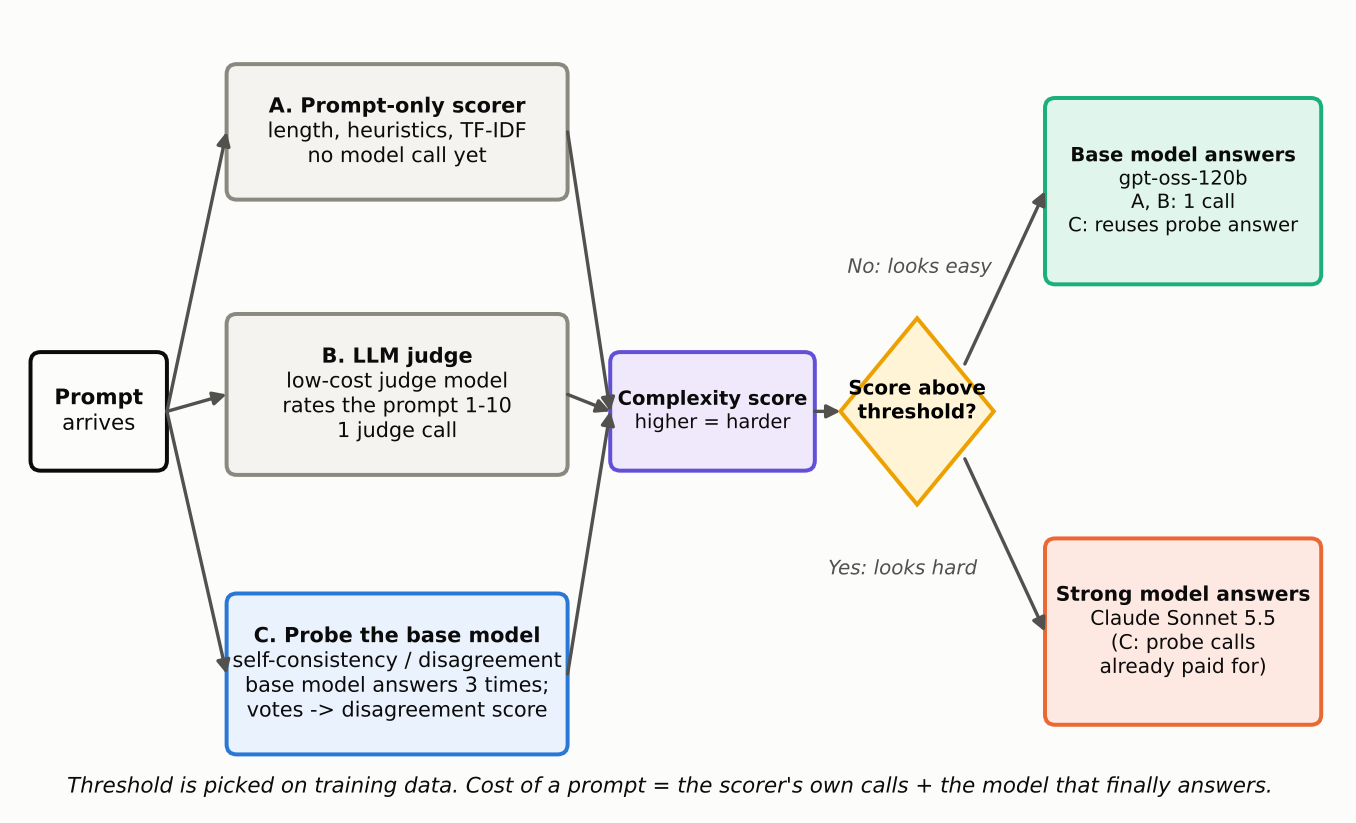
\includegraphics[width=\textwidth]{figs/fig_flow_part1_routing_paper.png}
\caption{Routing one prompt. Three kinds of scorer feed the same threshold. Prompt-only scorers (A) make no model call before the decision; an LLM judge (B) makes one; probe scorers (C) query the base model first and reuse its answer if the prompt stays on it.}\label{fig:flow_route}
\end{figure}

\begin{figure}[!htbp]
\centering
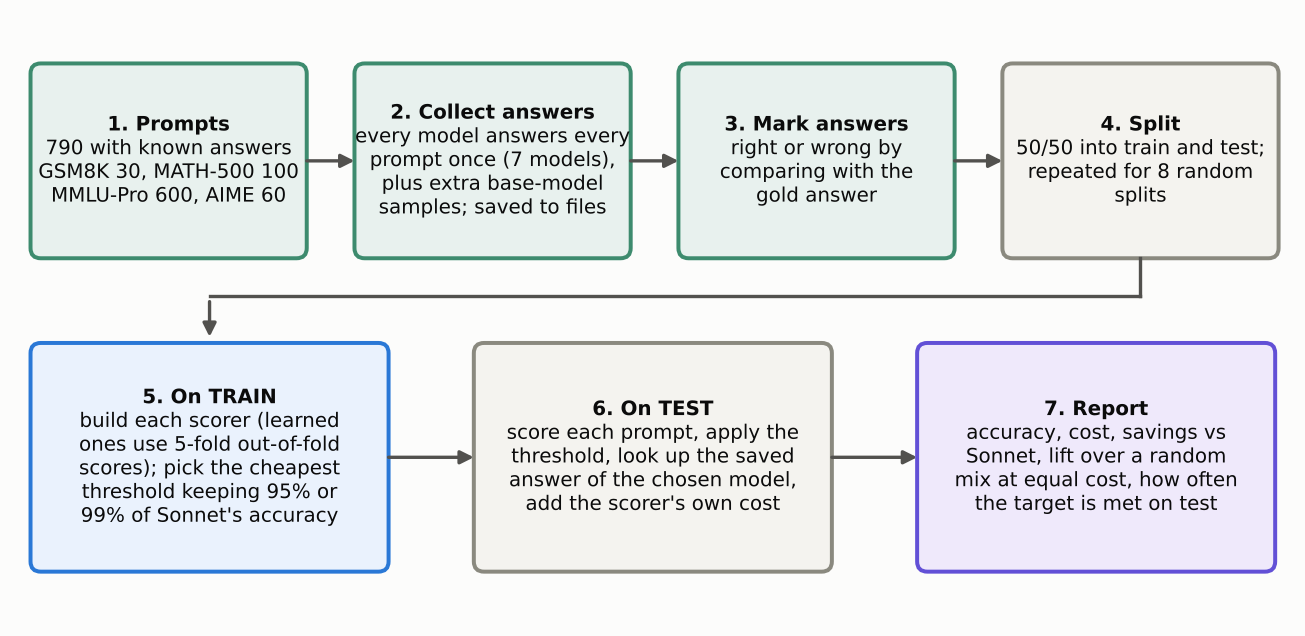
\includegraphics[width=\textwidth]{figs/fig_flow_part2_evaluation_paper.png}
\caption{Offline evaluation. Every model answers every prompt once and the answers and costs are cached; routers are then simulated on a held-out test half using the saved answers of whichever model they choose, with the scorer's own cost added.}\label{fig:flow_eval}
\end{figure}

\section{Results}
\subsection{Headroom is large}
Tables~\ref{tab:ref_full} and~\ref{tab:ref_mmlu} show that always using gpt-oss-120b costs 95--97\% less than Sonnet but loses 12.5--13.4 points of accuracy. An oracle that picks the cheapest of the two models that answers correctly costs 75\% less than Sonnet (USD 0.084 versus 0.333 per 100 prompts) and is more accurate (93.8\% versus 91.8\%; 92.1\% versus 89.6\% on MMLU-Pro). Relative to a random mix at equal cost, perfect difficulty information is worth roughly $+12$ points. The same information is available to a threshold router only through a score, and the best score for this pair puts the prompts where the base model is wrong and Sonnet is right first (``oracle for this pair'' in Table~\ref{tab:ci}); it saves about 80\% at the 95\% target with lift of about $+8$ points.

\begin{table}[!htbp]
\centering\small
\caption{Reference policies on the full mixed set (mean of 8 splits).}\label{tab:ref_full}
\begin{tabular}{lrrr}
\toprule
Policy & Acc.\ (\%) & USD/100 prompts & Savings vs.\ Sonnet (\%) \\
\midrule
Always gpt-oss-120b & 79.3 & 0.016 & 95.1 \\
Always Claude Sonnet 5.5 & 91.8 & 0.333 & 0.0 \\
Always Claude Opus 5.5 (reference) & 94.5 & 0.738 & -121.8 \\
Oracle router & 93.8 & 0.084 & 74.8 \\
\bottomrule
\end{tabular}
\end{table}

\begin{table}[!htbp]
\centering\small
\caption{Reference policies on MMLU-Pro only (mean of 8 splits).}\label{tab:ref_mmlu}
\begin{tabular}{lrrr}
\toprule
Policy & Acc.\ (\%) & USD/100 prompts & Savings vs.\ Sonnet (\%) \\
\midrule
Always gpt-oss-120b & 76.2 & 0.011 & 96.5 \\
Always Claude Sonnet 5.5 & 89.6 & 0.297 & 0.0 \\
Always Claude Opus 5.5 (reference) & 93.0 & 0.638 & -114.8 \\
Oracle router & 92.1 & 0.073 & 75.5 \\
\bottomrule
\end{tabular}
\end{table}


\subsection{Prompt text carries weak difficulty signal; probes carry more}
Table~\ref{tab:signal} measures how well each score detects the failures that matter for this pair: prompts gpt-oss-120b gets wrong (AUC fail) and prompts where it is wrong and Sonnet is right (AUC gain). It uses all 787 prompts with out-of-fold scores for learned scorers, so there are no intervals; differences of a few hundredths should not be over-read. An earlier version of this table measured correlation with the share of all seven pool models that fail and AUC for the failures of Llama-3.1-8B. That mixes in the weak models' failures and makes a probe built from pool models look better than it is for this pair.

\begin{table}[!htbp]
\centering\small
\caption{Signal quality of lightweight scorers for the pair used in the routing experiments, computed on all prompts (learned scorers use 5-fold out-of-fold scores; no train/test split). Spearman and the first AUC are against gpt-oss-120b's own failures; the second AUC is for ``needs Sonnet'' (gpt-oss-120b wrong, Sonnet right). Calls = model calls needed before the routing decision.}\label{tab:signal}
\begin{tabular}{lcrrrrrr}
\toprule
 & & \multicolumn{3}{c}{Full set} & \multicolumn{3}{c}{MMLU-Pro} \\
\cmidrule(lr){3-5}\cmidrule(lr){6-8}
Scorer & Calls & $\rho$ & AUC fail & AUC gain & $\rho$ & AUC fail & AUC gain \\
\midrule
\multicolumn{8}{l}{\emph{Prompt characteristics (read the prompt only)}} \\
Prompt length & 0 & 0.24 & 0.67 & 0.68 & 0.20 & 0.64 & 0.68 \\
Heuristic features & 0 & 0.03 & 0.52 & 0.54 & $-$0.07 & 0.45 & 0.48 \\
TF-IDF ridge & 0 & 0.27 & 0.69 & 0.68 & 0.26 & 0.68 & 0.66 \\
LLM judge & 1 & 0.11 & 0.58 & 0.59 & 0.10 & 0.57 & 0.57 \\
\midrule
\multicolumn{8}{l}{\emph{Model behaviour (needs model answers)}} \\
Llama-3.1-8B output length & 1 & $-$0.12 & 0.42 & 0.45 & $-$0.05 & 0.47 & 0.46 \\
Disagreement (gpt-oss-120b vs 20b) & 2 & 0.35 & 0.75 & 0.80 & 0.37 & 0.75 & 0.79 \\
Self-consistency (3 votes) & 2 & 0.55 & 0.76 & 0.82 & 0.52 & 0.74 & 0.80 \\
Combiner + samples + subject & 2--3 & 0.44 & 0.82 & 0.86 & 0.42 & 0.79 & 0.84 \\
\midrule
\multicolumn{8}{l}{\emph{References}} \\
Oracle for this pair (not realisable) & -- & 0.44 & 0.82 & 1.00 & 0.43 & 0.79 & 1.00 \\
Random scores & 0 & 0.03 & 0.52 & 0.50 & 0.03 & 0.52 & 0.50 \\
\bottomrule
\end{tabular}
\end{table}


Scores computed from the prompt alone carry weak signal. TF-IDF regression and prompt length reach AUC of 0.67--0.69 for the base model's failures on the mixed set and 0.64--0.68 inside MMLU-Pro, the heuristic features are close to chance and the LLM judge, which reads only the prompt, reaches 0.58. Part of the mixed-set AUC is dataset recognition: AIME prompts are long and hard, GSM8K prompts short and easy. Probes that look at the base model's behaviour are stronger. Self-consistency has the highest rank correlation with the base model's failures ($\rho=0.55$) and AUC of 0.76 (0.82 for ``needs Sonnet''), cross-model disagreement is close behind in AUC (0.75) with lower correlation, and the combiner with sampled answers and subject is highest in AUC (0.82). These signals hold inside MMLU-Pro. The length of Llama-3.1-8B's answer does not help.

\subsection{What the routers achieve at the 95\% point}
Tables~\ref{tab:95_full} and~\ref{tab:95_mmlu} and Figures~\ref{fig:cost} and~\ref{fig:lift} compare routers. \emph{Self-consistency (3 votes)} takes gpt-oss-120b's greedy answer plus two samples at temperature 0.8 and escalates unless all three agree. On the full set it saves 50.6\% (sd 3.2) of Sonnet's cost at 3.4 points lower accuracy, with lift $+3.3$ points (sd 0.8), meeting the target in 8 of 8 splits. On MMLU-Pro alone it saves 56.6\%, loses 4.5 points, has lift $+3.3$ points, and meets the target in 4 of 8 splits. Disagreement between gpt-oss-120b and gpt-oss-20b saves 48.7\% with lift $+2.1$ points ($+1.6$ on MMLU-Pro); a learned combiner of disagreement, token counts, prompt length and answer type saves 49.0\% with lift $+2.4$ ($+2.6$ on MMLU-Pro). Two further combiner variants (adding sampled answers, and adding subject) are in Appendix~\ref{app:all}, together with the 99\% tables; they do not change the conclusions. Prompt length alone saves 54.6\% but at $-5.1$ points with large spread across splits (sd 13.9 points of savings), and has lift $+2.3$ ($+2.1$ on MMLU-Pro); TF-IDF has $+0.7$ and heuristic features $-0.9$. Using a perfect ranking of the pool-share difficulty with the same thresholds gives 58.2\% savings and lift $+3.7$. That ranking is not specific to this pair: it ranks by the share of seven models that fail, not by whether gpt-oss-120b fails and Sonnet succeeds. A ranking built from the pair's own outcomes gives 79.6\% savings and lift $+8.1$ (Table~\ref{tab:ci}), so self-consistency reaches about 60\% of the achievable savings and about a third of the achievable lift. An earlier version of this paper said self-consistency ``reaches most of what any score can achieve''; that was relative to the weaker ranking and is not supported.

The 8 splits behind Tables~\ref{tab:95_full} and~\ref{tab:95_mmlu} overlap, so their standard deviations understate the uncertainty. Table~\ref{tab:ci} repeats the full-set comparison over 100 splits and bootstraps over prompts. Self-consistency has lift $+2.8$ (95\% interval 1.5 to 4.2), prompt length $+1.8$ (0.6 to 3.1), disagreement $+1.5$ (0.2 to 2.7) and the combiner with sampled answers and subject $+1.4$ (0.2 to 2.7). Self-consistency beats that combiner (difference 1.4, interval 0.6 to 2.2) and TF-IDF (1.8, 0.2 to 3.3), but its advantage over prompt length (1.0, interval $-0.8$ to 2.7) and over disagreement (1.4, interval $-0.1$ to 2.7) cannot be separated from zero. We therefore present it as the best of several comparable probes, not as a clear winner. The LLM judge and heuristic features have negative lift.

\begin{table}[!htbp]
\centering\small
\caption{Routers at the 95\% target over 100 random 50/50 splits (full set, the paper's threshold rule). Intervals are 95\% prompt-level bootstrap intervals (4000 draws) on each prompt's average result over the splits in which it was in the test half. Held = share of splits in which test retention met 95\%. Savings are relative to always using Sonnet.}\label{tab:ci}
\begin{tabular}{lrrrr}
\toprule
Router & Savings (\%) [95\% CI] & Lift (pp) [95\% CI] & Retention (\%) & Held \\
\midrule
Self-consistency (3 votes) & 48.9 [43.2, 54.8] & 2.8 [1.5, 4.2] & 96.8 & 98\% \\
Disagreement (120b vs 20b) & 45.7 [40.6, 51.2] & 1.5 [0.2, 2.7] & 95.7 & 65\% \\
Combiner + samples + subject & 40.9 [35.2, 46.9] & 1.4 [0.2, 2.7] & 96.3 & 91\% \\
Prompt length & 50.3 [46.0, 54.4] & 1.8 [0.6, 3.1] & 95.3 & 66\% \\
TF-IDF ridge & 42.4 [39.4, 45.6] & 1.1 [0.1, 2.0] & 95.7 & 67\% \\
Heuristic features & 26.7 [23.2, 30.4] & $-$0.7 [$-$1.9, 0.5] & 95.8 & 70\% \\
LLM judge & 21.2 [18.5, 24.1] & $-$1.2 [$-$2.3, $-$0.2] & 95.9 & 51\% \\
\midrule
Oracle difficulty (pool share; paper's earlier ceiling) & 58.0 [53.0, 63.1] & 3.5 [2.1, 4.9] & 96.4 & 89\% \\
Oracle for this pair (base wrong, Sonnet right) & 79.6 [75.5, 83.4] & 8.1 [6.7, 9.4] & 98.5 & 100\% \\
Random scores & 32.7 [32.0, 33.4] & $-$0.2 [$-$0.4, $-$0.0] & 95.5 & 69\% \\
\bottomrule
\end{tabular}
\end{table}


\begin{table}[!htbp]
\centering\small
\caption{Routers at the 95\% operating point, full mixed set. Mean over 8 train/test splits (standard deviation in parentheses). Savings and accuracy difference are relative to always using Sonnet; ``Splits at target'' counts splits where test retention of Sonnet's accuracy met the target; lift is accuracy above a random mix of the two models at equal cost.}\label{tab:95_full}
\begin{tabular}{lrrrrr}
\toprule
Router & Savings (\%) & Acc.\ diff (pp) & Retention (\%) & Splits at target & Lift (pp) \\
\midrule
Self-consistency (3 votes) & 50.6 (3.2) & -3.4 & 96.3 & 8/8 & 3.3 (0.8) \\
Disagreement (120b vs 20b) & 48.7 (3.0) & -4.3 & 95.3 & 5/8 & 2.1 (0.9) \\
Learned combiner & 49.0 (2.3) & -4.1 & 95.5 & 4/8 & 2.4 (0.6) \\
Prompt length & 54.6 (13.9) & -5.1 & 94.5 & 3/8 & 2.3 (0.5) \\
TF-IDF ridge & 46.7 (11.8) & -5.6 & 94.0 & 3/8 & 0.7 (0.6) \\
Heuristic features & 29.5 (3.6) & -4.8 & 94.8 & 3/8 & -0.9 (1.1) \\
Oracle difficulty (pool share) & 58.2 (3.2) & -4.0 & 95.6 & 5/8 & 3.7 (0.7) \\
Random scores & 43.8 (10.8) & -5.9 & 93.6 & 1/8 & -0.1 (0.9) \\
\bottomrule
\end{tabular}
\end{table}

\begin{table}[!htbp]
\centering\small
\caption{Routers at the 95\% operating point, MMLU-Pro only. Mean over 8 train/test splits (standard deviation in parentheses). Savings and accuracy difference are relative to always using Sonnet; ``Splits at target'' counts splits where test retention of Sonnet's accuracy met the target; lift is accuracy above a random mix of the two models at equal cost.}\label{tab:95_mmlu}
\begin{tabular}{lrrrrr}
\toprule
Router & Savings (\%) & Acc.\ diff (pp) & Retention (\%) & Splits at target & Lift (pp) \\
\midrule
Self-consistency (3 votes) & 56.6 (3.9) & -4.5 & 94.9 & 4/8 & 3.3 (0.8) \\
Disagreement (120b vs 20b) & 54.4 (11.8) & -6.0 & 93.3 & 1/8 & 1.6 (1.4) \\
Learned combiner & 49.6 (8.2) & -4.3 & 95.2 & 4/8 & 2.6 (1.0) \\
Prompt length & 53.6 (14.8) & -5.5 & 93.9 & 2/8 & 2.1 (1.4) \\
TF-IDF ridge & 51.5 (11.3) & -6.0 & 93.3 & 2/8 & 1.1 (1.1) \\
Heuristic features & 25.3 (7.1) & -4.6 & 94.9 & 5/8 & -1.0 (1.4) \\
Oracle difficulty (pool share) & 57.0 (7.4) & -4.4 & 95.1 & 5/8 & 3.5 (0.9) \\
Random scores & 26.7 (10.4) & -4.1 & 95.4 & 6/8 & -0.3 (1.1) \\
\bottomrule
\end{tabular}
\end{table}


\begin{figure}[!htbp]
\centering
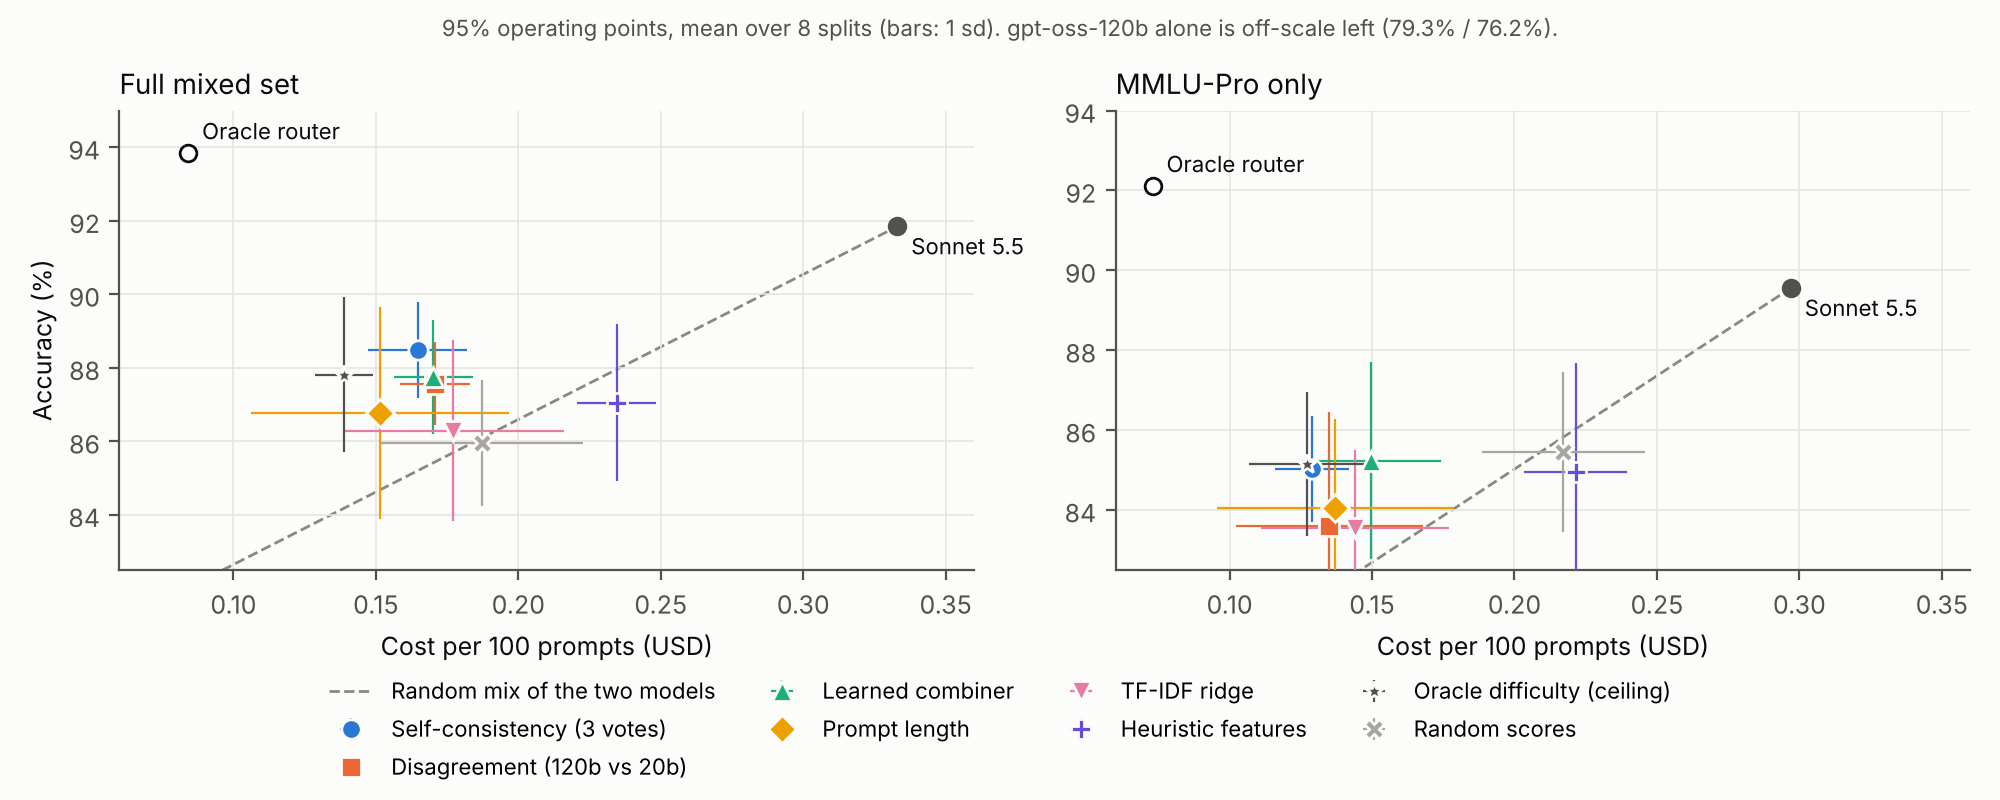
\includegraphics[width=\textwidth]{figs/fig1_cost_accuracy.png}
\caption{Cost versus accuracy at the 95\% operating points (mean over 8 splits; bars show one standard deviation). The dashed line is a random mix of gpt-oss-120b and Sonnet. gpt-oss-120b alone lies off-scale to the left (79.3\% and 76.2\%).}\label{fig:cost}
\end{figure}
\begin{figure}[!htbp]
\centering
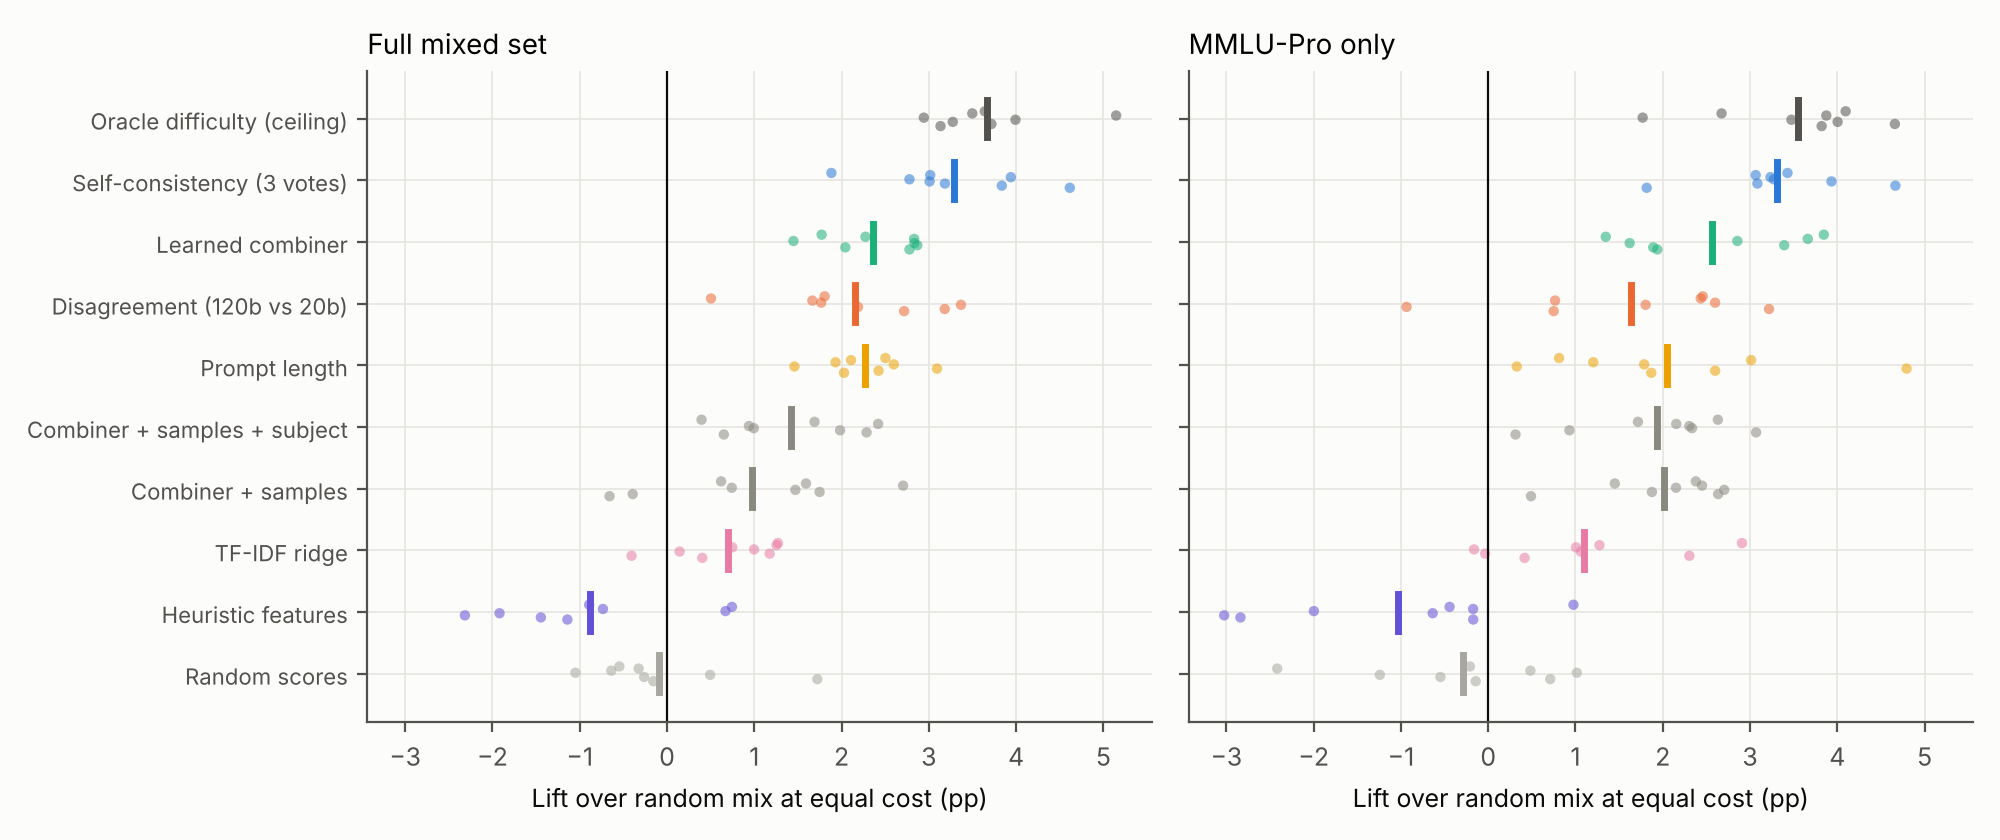
\includegraphics[width=\textwidth]{figs/fig2_lift_over_random_mix.png}
\caption{Lift over a random mix at equal cost at the 95\% operating point. Dots are individual splits; bars are means.}\label{fig:lift}
\end{figure}



Prompt length deserves a comment, since it comes within a point of the probes at no cost. Inside MMLU-Pro its AUC for the base model's failures is 0.64, so it looks like a weak but real signal in the original prompts (it fell to 0.54 on the fresh ones, Section~\ref{sec:fresh}); an earlier ``no explanation'' came from comparing it with the pool-share difficulty, where its correlation is 0.02. Two checks rule out simple artifacts. Escalated prompts are slightly \emph{more} expensive for Sonnet (USD 0.37 against 0.33 per 100 prompts for one split), so equal-cost comparison does not flatter it. But the length router is partly a dataset detector: it escalates about half of MMLU-Pro and 18\% of AIME, where the base model fails 25\% of the time (Table~\ref{tab:bench}), and it varies much more across splits (sd of savings 13.9 points against 3.2 for self-consistency).

\subsection{Quality targets chosen on training data do not transfer}\label{sec:rules}
At the 95\% point the threshold is the cheapest one that reaches 95\% of Sonnet's accuracy on the training half. It therefore sits at the boundary by construction, and with about 395 test prompts and one to two points of accuracy noise a good share of splits will fall short regardless of the scorer. Table~\ref{tab:rules} shows this. With a fine threshold grid every router except self-consistency meets the target in only 52--64\% of splits, including random scores (55\%) and the pair-specific oracle (64\%); with the coarser grid used in the main tables, random scores meet it in 69\% of splits and the oracle ranking in 89\%. With the 8 splits of the main tables the counts are noisier still (random scores 1 of 8). Self-consistency meets the target in 98\% of splits, but that reflects a coarse score rather than better transfer: it has only three distinct values (unanimous, two of three, all different), so the threshold jumps over the target and retention averages 96.8\%. The held-out misses say more about the thresholding rule than about the scorers, and we withdraw the earlier statement that no router is deployable on this basis.

Raising the training target by two points restores the target in 87--93\% of splits for most routers, but at a price. Savings fall from 55.8\% to 34.7\% for prompt length, from 51.6\% to 26.4\% for disagreement and from 47.7\% to 35.3\% for that combiner, while the pair-specific oracle keeps 80.8\%. Lift is largely preserved for that combiner (1.6) and the oracles but falls for length (1.2) and disagreement (0.4). Self-consistency cannot use a margin as it stands: the next feasible threshold escalates almost everything (2.9\% savings). It would need a finer score, for example a tie-break by answer length. A one-sided upper confidence bound on the training shortfall behaves like the two-point margin. We did not test conformal or Learn-then-Test procedures with finite-sample guarantees, which are the principled remedy and the natural next step.

\begin{table}[!htbp]
\centering\small
\caption{Effect of the threshold rule at the 95\% target (100 splits, full set). Each cell is savings (\%) / lift (pp) / share of splits in which the target was met. ``Target + 2 points'' picks the cheapest threshold reaching 97\% of Sonnet's training accuracy; ``upper confidence bound'' requires a one-sided 95\% normal upper bound on the training accuracy shortfall to stay within the allowed 5\%.}\label{tab:rules}
\resizebox{\textwidth}{!}{\begin{tabular}{lcccc}
\toprule
Router & Paper rule (11-step grid) & Same rule, 101-step grid & Target + 2 points & Upper confidence bound \\
\midrule
Self-consistency (3 votes) & 49.3 / 3.0 / 98\% & 49.3 / 3.0 / 98\% & 2.9 / $-$0.6 / 98\% & 9.5 / $-$0.1 / 98\% \\
Disagreement (120b vs 20b) & 45.8 / 1.6 / 65\% & 51.6 / 1.6 / 52\% & 26.4 / 0.4 / 91\% & 27.9 / 0.5 / 91\% \\
Combiner + samples + subject & 41.0 / 1.5 / 91\% & 47.7 / 1.3 / 54\% & 35.3 / 1.6 / 92\% & 36.4 / 1.6 / 92\% \\
Prompt length & 50.9 / 1.9 / 66\% & 55.8 / 1.9 / 55\% & 34.7 / 1.2 / 87\% & 36.4 / 1.3 / 86\% \\
Oracle difficulty (pool share) & 58.0 / 3.6 / 89\% & 63.9 / 3.4 / 61\% & 52.2 / 3.7 / 93\% & 54.1 / 3.7 / 92\% \\
Oracle for this pair & 79.6 / 8.1 / 100\% & 83.0 / 5.8 / 64\% & 80.8 / 7.3 / 89\% & 80.3 / 7.7 / 94\% \\
Random scores & 32.8 / $-$0.1 / 69\% & 37.8 / $-$0.0 / 55\% & 23.5 / $-$0.0 / 92\% & 24.9 / $-$0.1 / 88\% \\
\bottomrule
\end{tabular}}
\end{table}


At the 99\% target (Figure~\ref{fig:target}; full tables in Appendix~\ref{app:all}) no probe saves money reliably. Self-consistency escalates almost every prompt and pays for the probe on top, so it costs 11--14\% \emph{more} than always using Sonnet; its ``8/8 splits at target'' there is trivial because nearly everything goes to Sonnet. Cross-model disagreement and the learned combiner save 8--14\% on average with high variance and meet the target in only 2 or 3 of 8 splits.

\begin{figure}[!htbp]
\centering
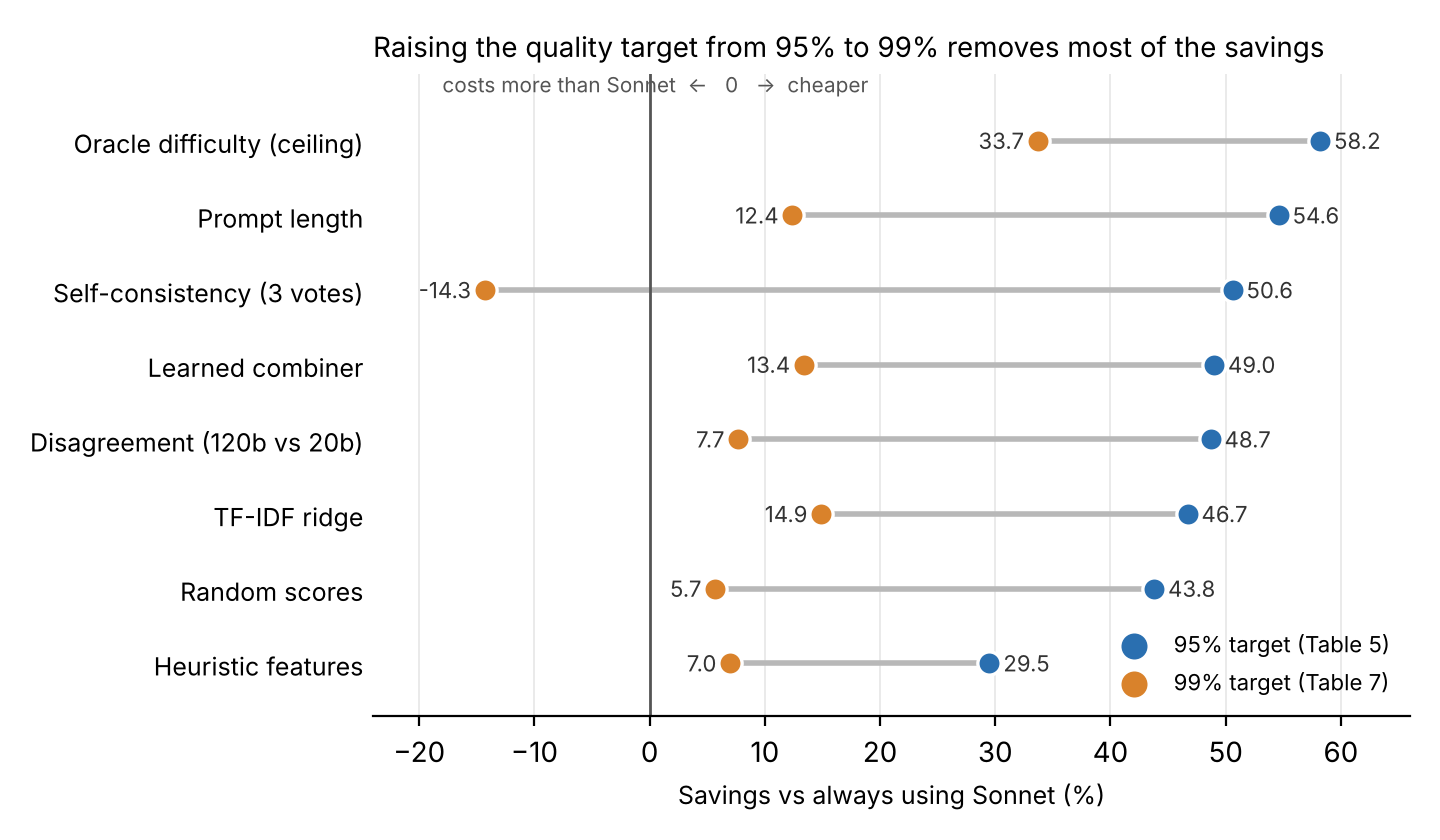
\includegraphics[width=\textwidth]{figs/fig_target_shift.png}
\caption{Savings relative to always using Sonnet at the 95\% and 99\% targets (full set, mean over 8 splits). Every router loses most of its savings at 99\%; self-consistency drops below zero, i.e.\ it costs more than Sonnet. MMLU-Pro results are in Table~\ref{tab:99_mmlu}.}\label{fig:target}
\end{figure}

\subsection{More samples do not help}
Tables~\ref{tab:k_full} and~\ref{tab:k_mmlu} and Figure~\ref{fig:votes} vary the number of votes. In the 8 splits of the tables lift is $+1.5$, $+3.3$ and $+1.5$ points for 2, 3 and 5 votes on the full set, and $-0.2$, $+3.3$ and $+1.9$ on MMLU-Pro. Two votes is unstable (sd of savings 34--37 points across splits); five votes is worse than three in 8 of 8 splits on the full set. Since five votes carry strictly more information than three, we read the three-vote peak as partly split-to-split noise of roughly 1.5 points; the vote count was chosen after seeing the results, and we report all three. All fail the 99\% target. Over 100 splits the lifts are $+0.6$, $+3.0$, $+2.3$ and $+1.7$ for 2, 3, 4 and 5 votes, so the peak at three votes persists but is steep, and two votes is unstable (sd of savings 37 points). To check how much of the peak is selection, we repeated the choice 60 times: split the prompts in half, pick the vote count with the best lift on one half (inner splits), and evaluate on the other half. Three votes is chosen in 43 of 60 partitions (four in 9, five in 5, two in 3), and the lift of the chosen count on the untouched half is $+2.6$ (sd 0.6), against $+3.0$ for the fixed choice. The vote count is therefore reasonably robust to selection within these prompts. Temperature and the disagreement partners cannot be re-selected without new samples and remain untested.

A structural limit is that some of gpt-oss-120b's errors are consistent. It makes 157 errors on 787 prompts; 41\% of them are identical across all three votes (8\% of all prompts), and the probe cannot see these. The probe flags 18\% of prompts and two thirds of the flagged prompts are errors; it finds 59\% of the errors. Unparsable answers do not drive this: only 14 prompts have an unparsable vote, and counting them as distinct votes, as one vote, or dropping them changes the flagged share between 16.8\% and 17.8\%. Parse failures concentrate on AIME (6.7\% of gpt-oss-120b's answers there, none elsewhere).

\begin{table}[!htbp]
\centering\small
\caption{Self-consistency with different numbers of votes, full set.}\label{tab:k_full}
\begin{tabular}{llrrrrr}
\toprule
Probe & Target & Savings (\%) & Acc.\ diff (pp) & Ret.\ (\%) & At target & Lift (pp) \\
\midrule
2 votes (K=1) & 95\% & 35.3 (37.3) & -3.6 & 96.1 & 3/8 & 1.5 (2.3) \\
2 votes (K=1) & 99\% & -9.7 (0.4) & +0.0 & 100.0 & 8/8 & -1.3 (0.2) \\
3 votes (K=2) & 95\% & 50.6 (3.2) & -3.4 & 96.3 & 8/8 & 3.3 (0.8) \\
3 votes (K=2) & 99\% & -14.3 (0.6) & +0.0 & 100.0 & 8/8 & -1.9 (0.2) \\
5 votes (K=4) & 95\% & 42.5 (7.7) & -4.1 & 95.5 & 4/8 & 1.5 (0.8) \\
5 votes (K=4) & 99\% & -17.0 (19.9) & -0.4 & 99.5 & 7/8 & -2.7 (1.5) \\
\bottomrule
\end{tabular}
\end{table}

\begin{table}[!htbp]
\centering\small
\caption{Self-consistency with different numbers of votes, MMLU-Pro only.}\label{tab:k_mmlu}
\begin{tabular}{llrrrrr}
\toprule
Probe & Target & Savings (\%) & Acc.\ diff (pp) & Ret.\ (\%) & At target & Lift (pp) \\
\midrule
2 votes (K=1) & 95\% & 10.7 (33.6) & -1.9 & 97.9 & 6/8 & -0.2 (1.5) \\
2 votes (K=1) & 99\% & -7.2 (0.4) & +0.0 & 100.0 & 8/8 & -1.0 (0.1) \\
3 votes (K=2) & 95\% & 56.6 (3.9) & -4.5 & 94.9 & 4/8 & 3.3 (0.8) \\
3 votes (K=2) & 99\% & -10.7 (0.5) & +0.0 & 100.0 & 8/8 & -1.5 (0.1) \\
5 votes (K=4) & 95\% & 50.0 (8.4) & -5.1 & 94.3 & 4/8 & 1.9 (1.2) \\
5 votes (K=4) & 99\% & -17.9 (0.8) & +0.0 & 100.0 & 8/8 & -2.5 (0.2) \\
\bottomrule
\end{tabular}
\end{table}


\begin{figure}[!htbp]
\centering
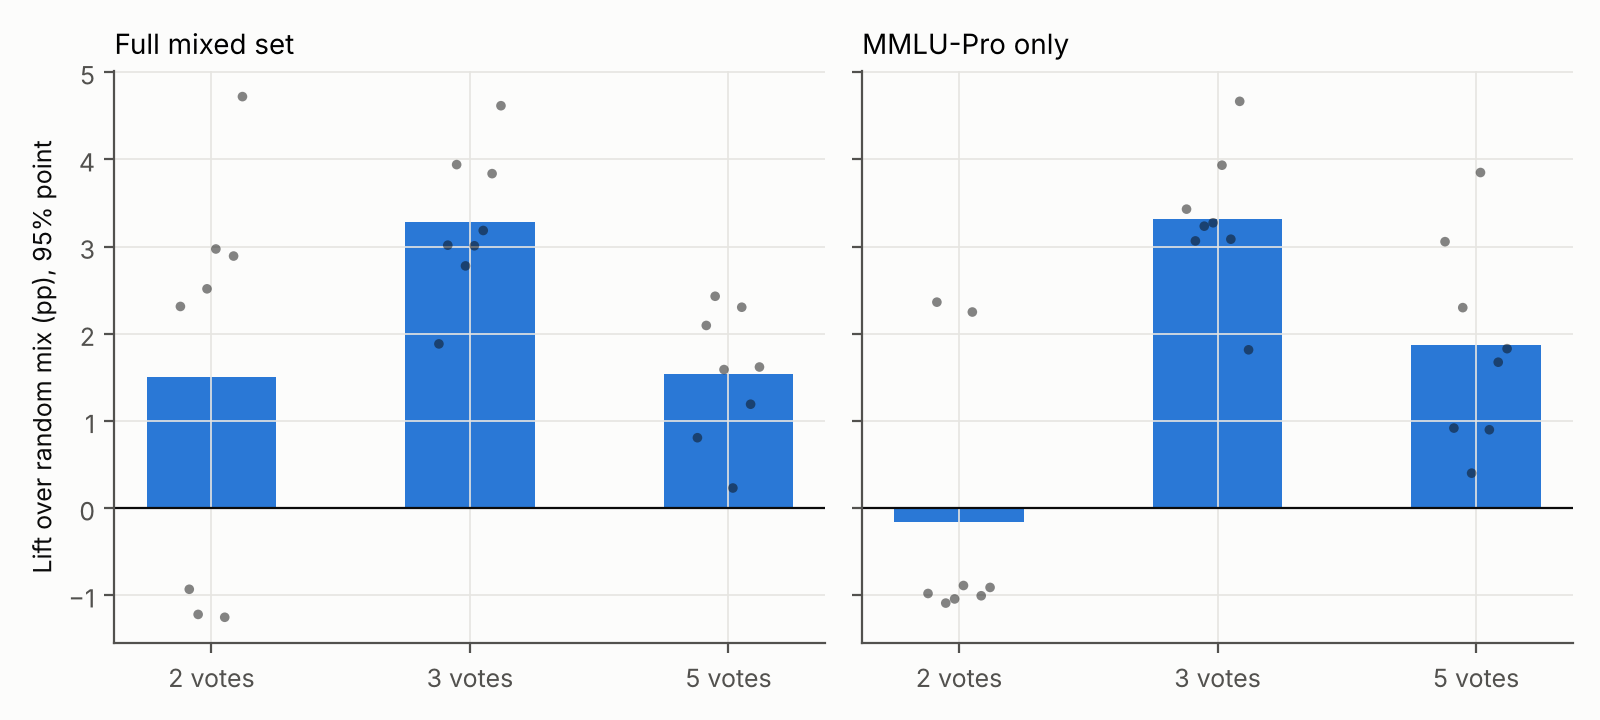
\includegraphics[width=0.8\textwidth]{figs/fig3_votes.png}
\caption{Self-consistency lift at the 95\% point for 2, 3 and 5 votes. Dots are individual splits.}\label{fig:votes}
\end{figure}

\subsection{Other model pairs}\label{sec:pairs}
To check how much depends on the gpt-oss-120b/Sonnet pair, we repeated the simulation for five further pairs using only the answers already cached (Table~\ref{tab:pairs}; complete tables in Appendix~\ref{app:all}). Three findings carry over. Headroom is large for every pair: ranking prompts by the pool-share difficulty saves 29--64\% at the 95\% target with lift between $+3.7$ and $+7.2$ points. This is the weaker ceiling; for the main pair a ranking from the pair's own outcomes roughly doubles the lift (Table~\ref{tab:ci}), and we did not recompute it for the other pairs. Prompt-only scorers stay weak: the best of length, TF-IDF and heuristics gives lift between $+0.4$ and $+2.4$ points, and only prompt length on the two gpt-oss-120b pairs ($+2.3$, $+2.4$) comes close to the probes, with large spread across splits. No router holds a 99\% target cheaply for any pair (Table~\ref{tab:pairs_99}).

What does not carry over is which probe works. Disagreement with a second model is the best realistic router for the two Qwen3-235B pairs ($+3.2$ and $+5.1$ points), but gives no lift when the base is Llama-3.3-70B or gpt-oss-20b ($0.0$ in both). Self-consistency could be tested only for gpt-oss-120b, and on the Opus pair its savings vary widely across splits (sd 32 points) and it meets the target in 4 of 8. The disagreement partner differs by pair and was chosen by us, so a stronger partner, not only a different base, may explain the better Qwen results. We did not test other partners.

\begin{table}[!htbp]
\centering\small
\caption{Other base/strong pairs at the 95\% target, full set. Each cell is lift over a random mix in points, then (savings relative to the strong model, splits at target out of 8). Mean over 8 splits. Self-consistency needs sampled answers, which we collected only for gpt-oss-120b. The disagreement probe pairs each base model with a partner chosen by us (gpt-oss-20b for gpt-oss-120b, gpt-oss-120b for Qwen3-235B, Llama-3.1-8B for Llama-3.3-70B and gpt-oss-20b). ``Best prompt-only'' is the best of prompt length, TF-IDF and heuristic features for that pair. Complete tables are in Appendix~\ref{app:all}.}\label{tab:pairs}
\begin{tabular}{lllll}
\toprule
Base $\to$ strong & Oracle (ceiling) & Self-consistency & Disagreement & Best prompt-only \\
\midrule
gpt-oss-120b $\to$ Sonnet 5.5 & +3.7 (58\%, 5/8) & +3.3 (51\%, 8/8) & +2.1 (49\%, 5/8) & Length +2.3 \\
gpt-oss-120b $\to$ Opus 5.5 & +5.8 (64\%, 5/8) & +3.7 (46\%, 4/8) & +2.6 (52\%, 2/8) & Length +2.4 \\
Qwen3-235B $\to$ Sonnet 5.5 & +5.2 (44\%, 7/8) & n/a & +3.2 (37\%, 6/8) & Heuristic +1.1 \\
Qwen3-235B $\to$ Opus 5.5 & +7.2 (50\%, 8/8) & n/a & +5.1 (49\%, 5/8) & Length +0.6 \\
Llama-3.3-70B $\to$ Sonnet 5.5 & +7.1 (29\%, 7/8) & n/a & 0.0 (15\%, 5/8) & Heuristic +0.4 \\
gpt-oss-20b $\to$ Sonnet 5.5 & +4.8 (45\%, 4/8) & n/a & 0.0 (23\%, 4/8) & Length +1.6 \\
\bottomrule
\end{tabular}
\end{table}


\subsection{Where the savings come from}
Table~\ref{tab:bench} splits the 95\% results by benchmark. Most of the savings come from MMLU-Pro, where self-consistency escalates 20\% of prompts and recovers about 70\% of the gap between gpt-oss-120b and Sonnet (85.5\% against 76.9\% and 89.1\%) at 46\% of Sonnet's cost. On AIME, where the base model fails 25\% of the time, the probe escalates 41\% and reaches 95.0\% against Sonnet's 96.7\%, but cost is still 84\% of Sonnet's. On MATH-500 and GSM8K the base model is already close to Sonnet and there is little to gain. Prompt length escalates only 18\% of AIME and loses accuracy there (78.6\%), which is the dataset-recognition effect mentioned above. The mixed benchmark therefore helps routers that can recognise the benchmark, and the MMLU-Pro-only tables are the cleaner test.

\begin{table}[!htbp]
\centering\small
\caption{Results by benchmark at the 95\% target (full set, 100 splits, paper threshold rule, prompts pooled by benchmark). Share escalated is the percentage of prompts sent to Sonnet; accuracy is the router's accuracy. Always-base and always-Sonnet accuracy are shown for reference.}\label{tab:bench}
\begin{tabular}{llrrrrr}
\toprule
Benchmark (n) & Router & Escalated (\%) & Accuracy (\%) & gpt-oss-120b & Sonnet & Cost / Sonnet \\
\midrule
MMLU-Pro (597) & Self-consistency & 20 & 85.5 & 76.9 & 89.1 & 46\% \\
 & Disagreement & 24 & 84.4 & 76.9 & 89.1 & 49\% \\
 & Prompt length & 51 & 85.8 & 76.9 & 89.1 & 60\% \\
\addlinespace
AIME (60) & Self-consistency & 41 & 95.0 & 75.0 & 96.7 & 84\% \\
 & Disagreement & 58 & 95.4 & 75.0 & 96.7 & 89\% \\
 & Prompt length & 18 & 78.6 & 75.0 & 96.7 & 31\% \\
\addlinespace
MATH-500 (100) & Self-consistency & 6 & 100.0 & 98.0 & 100.0 & 26\% \\
 & Disagreement & 11 & 99.3 & 98.0 & 100.0 & 29\% \\
 & Prompt length & 8 & 98.9 & 98.0 & 100.0 & 20\% \\
\addlinespace
GSM8K (30) & Self-consistency & 5 & 96.7 & 93.3 & 100.0 & 18\% \\
 & Disagreement & 0 & 93.3 & 93.3 & 100.0 & 6\% \\
 & Prompt length & 0 & 93.3 & 93.3 & 100.0 & 4\% \\
\addlinespace
\bottomrule
\end{tabular}
\end{table}


\subsection{Held-out check on fresh prompts}\label{sec:fresh}
Because the pair, vote count, temperature and partners were fixed on the original prompts, we collected 618 fresh prompts with no prompt text in common with the original set and ran the frozen configuration once. They come from three of the four benchmarks (300 MMLU-Pro, 218 MATH-500 and 100 GSM8K); no unused AIME problems were left, so the fresh set has none. The configuration was written down before collection: same pair, three-vote self-consistency at temperature 0.8, gpt-oss-20b as the disagreement partner, the same judge model, the 95\% target with and without a two-point margin, and thresholds fitted on the original 787 prompts only (raw score cut-offs, so nothing is fitted on the fresh prompts). We added two probes for the base model, a verbalised-confidence probe and a log-probability probe, and an embedding classifier (a small sentence encoder with logistic regression trained on the original prompts' base-model failures; this is in the spirit of classifier routers such as RouteLLM's, not RouteLLM itself). The log-probability probe could not be evaluated: 36\% of fresh prompts returned no log-probabilities from the provider. One fresh prompt received no judge rating. Four prompts lack an answer from at least one of the seven models (one of them from gpt-oss-120b) and are dropped, leaving 614 (297 MMLU-Pro, 217 MATH-500, 100 GSM8K).

Table~\ref{tab:fresh} gives the result. The fresh mix is easier for the base model: MMLU-Pro is 48\% of the prompts against 76\% originally and there is no AIME, so the pair-specific oracle escalates only 3.4\% of them and reaches lift $+3.0$, against about $+8$ on the original prompts. Lifts in points are therefore smaller for reasons unrelated to the routers and should be read against that ceiling; this is not a replication on the same mix. Self-consistency saves 64.0\% at 97.0\% retention and has lift $+1.9$ (interval 0.7 to 3.1), about 63\% of the oracle lift. It is lower than the original $+2.8$, as expected when a choice was selected on the original prompts, but clearly above zero. Disagreement replicates ($+1.6$; original $+1.5$) and the LLM judge and heuristic features stay at or below zero. Prompt length does not replicate: $+0.5$, with an interval that includes zero, against $+1.8$ originally. The embedding classifier has lift $+2.0$ (0.6 to 3.3) and saves 64.9\%, with no model call before the routing decision, and verbalised confidence is weaker ($+0.6$, interval $-0.6$ to 1.8).

Self-consistency still has no demonstrated lead. Its paired lift difference is $+0.3$ over disagreement (interval $-1.1$ to 1.9), $-0.1$ against the embedding classifier ($-1.8$ to 1.7), $+1.4$ over prompt length ($-0.4$ to 3.2), $+0.9$ over TF-IDF ($-1.0$ to 2.7) and $+1.3$ over verbalised confidence ($-0.2$ to 2.9); it beats only the judge and the heuristic features. With the two-point margin, self-consistency again escalates every prompt ($-11.4$\% savings), because its score has too few levels; the embedding classifier ($+1.7$, savings 50.4\%) and verbalised confidence ($+1.4$, savings 44.2\%) keep positive lift with margins. Every router reached the 95\% target in this single run, with thresholds fitted on 787 rather than about 395 prompts. One run per router says little about how often a target is met, so this does not settle the transfer question raised in Section~\ref{sec:rules}. All of this is in distribution: the fresh prompts come from the same four benchmarks as the training prompts, and the embedding classifier in particular was trained on labels from them.

\begin{table}[!htbp]
\centering\small
\caption{Held-out check on 614 fresh prompts with all thresholds fixed on the original 787 prompts (one run, no tuning on the fresh prompts). Intervals are 95\% bootstrap intervals over fresh prompts. The first group of columns uses the paper's rule (cheapest cut-off reaching 95\% of Sonnet's accuracy on the original prompts); the last two use a 97\% training target. Logprob-based confidence is omitted: 36\% of fresh prompts (and 41\% of the original ones) returned no logprobs.}\label{tab:fresh}
\resizebox{\textwidth}{!}{\begin{tabular}{lrrrrrr}
\toprule
 & \multicolumn{4}{c}{95\% target} & \multicolumn{2}{c}{97\% training target} \\
\cmidrule(lr){2-5}\cmidrule(lr){6-7}
Router & Savings (\%) [95\% CI] & Retention (\%) & Escalated (\%) & Lift (pp) [95\% CI] & Savings (\%) & Lift (pp) [95\% CI] \\
\midrule
Self-consistency (3 votes) & 64.0 [58.5, 69.8] & 97.0 & 12 & 1.9 [0.7, 3.1] & $-$11.4 & $-$0.8 [$-$1.1, $-$0.5] \\
Disagreement (120b vs 20b) & 66.4 [60.8, 72.2] & 96.5 & 13 & 1.6 [0.4, 2.8] & 37.7 & 0.3 [$-$0.8, 1.4] \\
Embedding classifier (MiniLM + logistic) & 64.9 [60.0, 69.8] & 97.0 & 23 & 2.0 [0.6, 3.3] & 50.4 & 1.7 [0.5, 2.9] \\
Verbalised confidence & 56.9 [51.7, 62.3] & 96.2 & 20 & 0.6 [$-$0.6, 1.8] & 44.2 & 1.4 [0.3, 2.6] \\
TF-IDF ridge & 63.5 [58.7, 68.3] & 96.2 & 24 & 1.0 [$-$0.1, 2.3] & 58.0 & 0.6 [$-$0.6, 1.9] \\
Prompt length & 60.8 [55.8, 65.8] & 95.8 & 25 & 0.5 [$-$0.7, 1.7] & 45.6 & 0.7 [$-$0.5, 1.9] \\
LLM judge & 42.3 [37.7, 47.3] & 96.2 & 36 & $-$0.5 [$-$1.7, 0.7] & 23.0 & $-$0.8 [$-$1.9, 0.3] \\
Heuristic features & 43.0 [38.3, 47.8] & 96.5 & 38 & $-$0.1 [$-$1.3, 1.1] & 34.8 & $-$0.1 [$-$1.2, 1.1] \\
\midrule
Oracle for this pair & 90.3 [87.1, 93.2] & 96.2 & 3 & 3.0 [1.9, 4.2] & 88.0 & 4.1 [2.8, 5.5] \\
Random scores & 34.2 [29.6, 38.9] & 96.5 & 63 & $-$0.8 [$-$1.9, 0.3] & 22.2 & $-$0.8 [$-$1.8, 0.1] \\
\bottomrule
\end{tabular}}
\end{table}


Table~\ref{tab:fresh_bench} breaks the fresh result down by benchmark. On MMLU-Pro the gap between the two models is the same as originally (76.4\% for gpt-oss-120b and 88.2\% for Sonnet, against 76.9\% and 89.1\%), while on MATH-500 and GSM8K it is only two to three points, so the smaller overall gap and the smaller lifts come from the mix, not from the routers. Inside MMLU-Pro, the AUC for the base model's 70 failures is 0.69 for self-consistency, 0.70 for disagreement, 0.68 for the embedding classifier, 0.67 for verbalised confidence, 0.54 for prompt length and 0.51 for the LLM judge; with this few failures the differences among the first four are within noise. The embedding classifier is therefore not only recognising the benchmark. Prompt length loses its inside-MMLU-Pro signal (0.64 originally), which agrees with its lift not replicating. The routers spend their escalations differently on MMLU-Pro: self-consistency sends 21\% of prompts to Sonnet and the embedding classifier 45\%, which recovers more of the accuracy gap (84.5\% against 82.5\%) at a higher cost.

\begin{table}[!htbp]
\centering\small
\caption{Fresh-prompt results by benchmark at the 95\% target (thresholds fixed on the original prompts, one run). Escalated is the percentage of prompts sent to Sonnet; Cost is the router's cost as a percentage of always using Sonnet on those prompts. MATH-500 and GSM8K have only 7 and 6 base-model errors, so their rows are very noisy.}\label{tab:fresh_bench}
\begin{tabular}{llrrrrr}
\toprule
Benchmark (n) & Router & Escalated (\%) & Accuracy (\%) & gpt-oss-120b & Sonnet & Cost (\%) \\
\midrule
MMLU-Pro (297) & Self-consistency & 21 & 82.5 & 76.4 & 88.2 & 42 \\
 & Disagreement & 21 & 81.8 & 76.4 & 88.2 & 41 \\
 & Embedding classifier & 45 & 84.5 & 76.4 & 88.2 & 52 \\
 & Verbalised confidence & 32 & 82.2 & 76.4 & 88.2 & 53 \\
 & Prompt length & 49 & 82.8 & 76.4 & 88.2 & 58 \\
\addlinespace
MATH-500 (217) & Self-consistency & 5 & 99.5 & 96.8 & 99.5 & 32 \\
 & Disagreement & 6 & 99.5 & 96.8 & 99.5 & 26 \\
 & Embedding classifier & 4 & 97.7 & 96.8 & 99.5 & 12 \\
 & Verbalised confidence & 12 & 98.6 & 96.8 & 99.5 & 34 \\
 & Prompt length & 3 & 97.2 & 96.8 & 99.5 & 12 \\
\addlinespace
GSM8K (100) & Self-consistency & 2 & 96.0 & 94.0 & 96.0 & 13 \\
 & Disagreement & 1 & 95.0 & 94.0 & 96.0 & 6 \\
 & Embedding classifier & 1 & 94.0 & 94.0 & 96.0 & 4 \\
 & Verbalised confidence & 3 & 94.0 & 94.0 & 96.0 & 9 \\
 & Prompt length & 1 & 93.0 & 94.0 & 96.0 & 5 \\
\addlinespace
\bottomrule
\end{tabular}
\end{table}


\FloatBarrier
\section{Claims and limitations}
\textbf{What the results support.} (1) Headroom is large: a router that knew where the base model fails and Sonnet succeeds would save about 80\% of Sonnet's cost at higher accuracy. (2) Simple prompt features are a weak difficulty signal here (AUC 0.5--0.7 for the base model's failures) and a low-cost LLM judge does not change that, but a small embedding classifier trained on labelled base-model failures matched our best probe on fresh prompts from the same benchmarks. (3) Probing the base model works somewhat better for gpt-oss-120b: three-vote self-consistency saves about 49\% at about 96\% retention and is $+2.8$ points above a random mix, but its lead over prompt length, cross-model disagreement and the embedding classifier is not statistically separable, on the original prompts or on 614 fresh ones. For the Qwen3-235B pairs, disagreement with a second model gives $+3$ to $+5$ points; for Llama-3.3-70B and gpt-oss-20b as base it gave none. (4) Most of the headroom stays unused (about one third of the achievable lift), and a threshold picked on training data to hit a quality target frequently misses it on held-out data, mostly because of the thresholding rule; a safety margin repairs that at a cost of 12 to 25 points of savings. The results do \emph{not} show that a router holds Sonnet-level quality at low cost, that a probe beats prompt length by a wide margin, that one probe is best across model pairs, or that they transfer to other benchmarks or agentic tasks.

\textbf{Limitations.} \emph{Selection on the evaluation data.} The base/strong pair, the vote count, the sampling temperature, the disagreement partners and the 95\%/99\% targets were fixed after seeing results on these 787 prompts. The fresh-prompt run (Section~\ref{sec:fresh}) tests the frozen configuration once on 614 new prompts from the same benchmarks; it shrinks the self-consistency lift from $+2.8$ to $+1.9$ and removes prompt length's lift, so the original numbers should be read as optimistic. The fresh prompts come from three of the same benchmarks (no AIME), with a different mix, so they say nothing about other benchmarks, and the temperature and partners were still not varied. \emph{Statistics.} The 8 splits overlap, and the bootstrap in Table~\ref{tab:ci} resamples prompts but not the choice of pair or temperature; the pair study has one run per pair. \emph{Scope.} One main base/strong pair (the strong model is Claude Sonnet 5.5 only because it was in our pool) and five further pairs checked on cached answers, where self-consistency was possible only for gpt-oss-120b and the disagreement partners were chosen by us; four public benchmarks with numeric or letter answers, MMLU-Pro being 76\% of prompts, which may be contaminated for both models; no coding, free-form, long-context, multilingual or agentic work, where agreement between samples is harder to define. \emph{Baselines.} We ran an embedding classifier and a verbalised-confidence probe on the fresh prompts, but no published router (RouteLLM, UniRoute, R2-Router) and no activation probe; the token-probability probe could not be evaluated because 36\% of fresh prompts returned no log-probabilities. The embedding classifier is a small, in-distribution stand-in for a learned router, not a reproduction of any of them. \emph{Cost and latency.} Prices are an OpenRouter snapshot. Sampled calls were collected separately from the greedy calls and priced per call from reported usage, and the greedy answer is charged once. We did not measure latency: three samples plus escalation add sequential delay. Reasoning-effort variation of gpt-oss-120b was not studied. \emph{Combiner.} The learned combiner is trained and evaluated in-distribution with cross-fitting, with scores fixed across splits. Model identifiers, providers and prices can change; the cache was collected on specific dates.

\textbf{Broader impact.} Escalating fewer prompts to the strong model lowers cost but, in our data, also lowers accuracy by about three points at the operating points we report. For sensitive uses (medical, legal, safety) that trade-off, and the fact that about 40\% of the base model's errors are consistent and therefore invisible to a sampling probe, argue for conservative thresholds and human review. The experiments used public benchmarks and no personal data.

\FloatBarrier
\section{Conclusion}
We compared several cheap difficulty scorers under one fixed router that chooses between a base model (gpt-oss-120b) and a strong model (Claude Sonnet 5.5), using cached model answers so every router sees the same outputs. The headroom is large: a router that knew where the base model fails and Sonnet succeeds would save about 80\% of the strong model's cost at higher accuracy. Scorers computed from the prompt alone, including an LLM judge, carried weak signal. Probing the base model worked better: three-vote self-consistency saved about half of the strong model's cost at about 3 points lower accuracy and $+2.8$ points above a random mix at equal cost, although this is not statistically separable from prompt length or cross-model disagreement. Most of the headroom stayed unused, because many of the base model's errors are consistent and invisible to a probe, and because a quality target chosen on training data is often missed on held-out data. Much of that miss is produced by the thresholding rule, and a safety margin repairs it at a substantial cost in savings. A held-out run on 614 fresh prompts reproduced a positive lift for self-consistency ($+1.9$) and disagreement ($+1.6$) but not for prompt length, and showed a small embedding classifier trained on the original prompts matching self-consistency ($+2.0$) with no model call, so the evidence does not single out a sampling probe. No probe was cost-effective at a 99\% target. The main pair was checked against five others on cached answers: headroom and the weakness of prompt-only scorers carried over, while the best probe depended on the pair. These conclusions come from four exam-style benchmarks and 787 prompts, with several choices made on the same prompts. The next steps are published trained-router and activation baselines, other benchmarks and model pools, risk-controlled thresholds with finite-sample guarantees, and prompts beyond exam-style benchmarks.

\subsection*{Reproducibility}
The experiment has four stages: building the prompt file, collecting and caching every model's answers, building the scorers, and simulating routers on the cache over several train/test splits. All scripts, the prompt file and the cached answers will be released at \textbf{[repository URL]}. The API key is not included in the release.

\appendix
\section{Complete router tables}\label{app:all}
\begin{table}[!htbp]
\centering\small
\caption{Complete version, including both combiner variants. Routers at the 95\% operating point, full mixed set. Mean over 8 train/test splits (standard deviation in parentheses). Savings and accuracy difference are relative to always using Sonnet; ``Splits at target'' counts splits where test retention of Sonnet's accuracy met the target; lift is accuracy above a random mix of the two models at equal cost.}\label{tab:95_full_all}
\begin{tabular}{lrrrrr}
\toprule
Router & Savings (\%) & Acc.\ diff (pp) & Retention (\%) & Splits at target & Lift (pp) \\
\midrule
Self-consistency (3 votes) & 50.6 (3.2) & -3.4 & 96.3 & 8/8 & 3.3 (0.8) \\
Disagreement (120b vs 20b) & 48.7 (3.0) & -4.3 & 95.3 & 5/8 & 2.1 (0.9) \\
Learned combiner & 49.0 (2.3) & -4.1 & 95.5 & 4/8 & 2.4 (0.6) \\
Combiner + samples & 45.4 (8.8) & -5.0 & 94.5 & 6/8 & 1.0 (1.1) \\
Combiner + samples + subject & 44.3 (5.9) & -4.4 & 95.2 & 5/8 & 1.4 (0.8) \\
Prompt length & 54.6 (13.9) & -5.1 & 94.5 & 3/8 & 2.3 (0.5) \\
TF-IDF ridge & 46.7 (11.8) & -5.6 & 94.0 & 3/8 & 0.7 (0.6) \\
Heuristic features & 29.5 (3.6) & -4.8 & 94.8 & 3/8 & -0.9 (1.1) \\
Oracle difficulty (pool share) & 58.2 (3.2) & -4.0 & 95.6 & 5/8 & 3.7 (0.7) \\
Random scores & 43.8 (10.8) & -5.9 & 93.6 & 1/8 & -0.1 (0.9) \\
\bottomrule
\end{tabular}
\end{table}

\begin{table}[!htbp]
\centering\small
\caption{Complete version, including both combiner variants. Routers at the 95\% operating point, MMLU-Pro only. Mean over 8 train/test splits (standard deviation in parentheses). Savings and accuracy difference are relative to always using Sonnet; ``Splits at target'' counts splits where test retention of Sonnet's accuracy met the target; lift is accuracy above a random mix of the two models at equal cost.}\label{tab:95_mmlu_all}
\begin{tabular}{lrrrrr}
\toprule
Router & Savings (\%) & Acc.\ diff (pp) & Retention (\%) & Splits at target & Lift (pp) \\
\midrule
Self-consistency (3 votes) & 56.6 (3.9) & -4.5 & 94.9 & 4/8 & 3.3 (0.8) \\
Disagreement (120b vs 20b) & 54.4 (11.8) & -6.0 & 93.3 & 1/8 & 1.6 (1.4) \\
Learned combiner & 49.6 (8.2) & -4.3 & 95.2 & 4/8 & 2.6 (1.0) \\
Combiner + samples & 52.2 (2.9) & -5.2 & 94.1 & 1/8 & 2.0 (0.7) \\
Combiner + samples + subject & 53.0 (3.0) & -5.5 & 93.9 & 1/8 & 1.9 (0.9) \\
Prompt length & 53.6 (14.8) & -5.5 & 93.9 & 2/8 & 2.1 (1.4) \\
TF-IDF ridge & 51.5 (11.3) & -6.0 & 93.3 & 2/8 & 1.1 (1.1) \\
Heuristic features & 25.3 (7.1) & -4.6 & 94.9 & 5/8 & -1.0 (1.4) \\
Oracle difficulty (pool share) & 57.0 (7.4) & -4.4 & 95.1 & 5/8 & 3.5 (0.9) \\
Random scores & 26.7 (10.4) & -4.1 & 95.4 & 6/8 & -0.3 (1.1) \\
\bottomrule
\end{tabular}
\end{table}

\begin{table}[!htbp]
\centering\small
\caption{Routers at the 99\% operating point, full mixed set. Mean over 8 train/test splits (standard deviation in parentheses). Savings and accuracy difference are relative to always using Sonnet; ``Splits at target'' counts splits where test retention of Sonnet's accuracy met the target; lift is accuracy above a random mix of the two models at equal cost.}\label{tab:99_full}
\begin{tabular}{lrrrrr}
\toprule
Router & Savings (\%) & Acc.\ diff (pp) & Retention (\%) & Splits at target & Lift (pp) \\
\midrule
Self-consistency (3 votes) & -14.3 (0.6) & +0.0 & 100.0 & 8/8 & -1.9 (0.2) \\
Disagreement (120b vs 20b) & 7.7 (7.0) & -1.3 & 98.6 & 2/8 & -0.4 (0.4) \\
Learned combiner & 13.4 (13.2) & -1.4 & 98.5 & 3/8 & 0.4 (1.1) \\
Combiner + samples & -0.6 (8.2) & -0.9 & 99.0 & 4/8 & -1.0 (0.5) \\
Combiner + samples + subject & -2.3 (3.8) & -0.7 & 99.2 & 7/8 & -1.0 (0.3) \\
Prompt length & 12.4 (6.8) & -0.8 & 99.1 & 5/8 & 0.9 (0.3) \\
TF-IDF ridge & 14.9 (9.7) & -1.2 & 98.7 & 3/8 & 0.8 (0.5) \\
Heuristic features & 7.0 (4.8) & -1.0 & 99.0 & 5/8 & -0.0 (0.6) \\
Oracle difficulty (pool share) & 33.7 (8.8) & -1.2 & 98.7 & 6/8 & 3.3 (0.6) \\
Random scores & 5.7 (6.8) & -1.0 & 98.9 & 4/8 & -0.3 (0.6) \\
\bottomrule
\end{tabular}
\end{table}

\begin{table}[!htbp]
\centering\small
\caption{Routers at the 99\% operating point, MMLU-Pro only. Mean over 8 train/test splits (standard deviation in parentheses). Savings and accuracy difference are relative to always using Sonnet; ``Splits at target'' counts splits where test retention of Sonnet's accuracy met the target; lift is accuracy above a random mix of the two models at equal cost.}\label{tab:99_mmlu}
\begin{tabular}{lrrrrr}
\toprule
Router & Savings (\%) & Acc.\ diff (pp) & Retention (\%) & Splits at target & Lift (pp) \\
\midrule
Self-consistency (3 votes) & -10.7 (0.5) & +0.0 & 100.0 & 8/8 & -1.5 (0.1) \\
Disagreement (120b vs 20b) & 10.2 (9.1) & -1.3 & 98.6 & 3/8 & 0.2 (0.6) \\
Learned combiner & 14.3 (13.5) & -1.4 & 98.4 & 3/8 & 0.6 (1.0) \\
Combiner + samples & 7.4 (13.9) & -1.6 & 98.2 & 2/8 & -0.5 (0.9) \\
Combiner + samples + subject & 3.6 (7.6) & -1.2 & 98.7 & 4/8 & -0.6 (0.6) \\
Prompt length & 11.1 (3.4) & -0.4 & 99.5 & 6/8 & 1.1 (0.4) \\
TF-IDF ridge & 15.5 (6.8) & -1.5 & 98.3 & 5/8 & 0.7 (0.8) \\
Heuristic features & 7.6 (6.1) & -1.1 & 98.8 & 4/8 & -0.0 (0.5) \\
Oracle difficulty (pool share) & 31.7 (2.6) & -0.9 & 99.0 & 4/8 & 3.5 (0.4) \\
Random scores & 0.8 (2.3) & -0.2 & 99.8 & 7/8 & -0.0 (0.1) \\
\bottomrule
\end{tabular}
\end{table}

\FloatBarrier
\begin{longtable}{lrrrrr}
\caption{Routers for every base/strong pair at the 95\% target, full set. Mean over 8 splits (standard deviation in parentheses). Rows within a pair are sorted by lift. Self-consistency exists only for gpt-oss-120b.}\label{tab:pairs_95}\\
\toprule
Router & Savings (\%) & Acc.\ diff (pp) & Retention (\%) & At target & Lift (pp) \\
\midrule
\endfirsthead
\toprule
Router & Savings (\%) & Acc.\ diff (pp) & Retention (\%) & At target & Lift (pp) \\
\midrule
\endhead
\multicolumn{6}{l}{\emph{gpt-oss-120b $\to$ Sonnet 5.5}} \\
Oracle difficulty (pool share) & 58.2 (3.2) & $-$4.0 & 95.6 & 5/8 & +3.7 (0.7) \\
Self-consistency (3 votes) & 50.6 (3.2) & $-$3.4 & 96.3 & 8/8 & +3.3 (0.8) \\
Prompt length & 54.6 (13.9) & $-$5.1 & 94.5 & 3/8 & +2.3 (0.5) \\
Disagreement & 48.7 (3.0) & $-$4.3 & 95.3 & 5/8 & +2.1 (0.9) \\
TF-IDF ridge & 46.7 (11.8) & $-$5.5 & 94.0 & 3/8 & +0.7 (0.6) \\
Random scores & 43.8 (10.8) & $-$5.9 & 93.6 & 1/8 & $-$0.1 (0.9) \\
Heuristic features & 29.5 (3.6) & $-$4.8 & 94.8 & 3/8 & $-$0.9 (1.1) \\
\midrule
\multicolumn{6}{l}{\emph{gpt-oss-120b $\to$ Opus 5.5}} \\
Oracle difficulty (pool share) & 63.7 (3.5) & $-$1.5 & 95.6 & 5/8 & +5.8 (0.6) \\
Self-consistency (3 votes) & 45.9 (32.2) & $-$1.3 & 95.8 & 4/8 & +3.7 (2.9) \\
Disagreement & 51.7 (12.1) & $-$2.8 & 94.3 & 2/8 & +2.6 (1.4) \\
Prompt length & 46.9 (12.8) & $-$2.4 & 94.7 & 3/8 & +2.4 (0.7) \\
TF-IDF ridge & 43.5 (12.3) & $-$3.3 & 93.7 & 3/8 & +1.0 (0.8) \\
Random scores & 36.7 (8.2) & $-$3.2 & 93.8 & 1/8 & $-$0.1 (0.8) \\
Heuristic features & 25.3 (5.6) & $-$2.5 & 94.6 & 3/8 & $-$1.1 (0.9) \\
\midrule
\multicolumn{6}{l}{\emph{Qwen3-235B $\to$ Sonnet 5.5}} \\
Oracle difficulty (pool share) & 43.9 (3.2) & $-$2.9 & 96.9 & 7/8 & +5.2 (1.1) \\
Disagreement & 37.3 (2.6) & $-$3.7 & 96.0 & 6/8 & +3.2 (0.8) \\
Heuristic features & 26.6 (3.6) & $-$3.8 & 95.9 & 5/8 & +1.1 (0.8) \\
TF-IDF ridge & 23.4 (6.3) & $-$4.1 & 95.5 & 5/8 & +0.2 (0.7) \\
Random scores & 23.7 (5.8) & $-$4.5 & 95.1 & 4/8 & $-$0.1 (0.7) \\
Prompt length & 20.9 (5.1) & $-$4.5 & 95.1 & 5/8 & $-$0.6 (0.6) \\
\midrule
\multicolumn{6}{l}{\emph{Qwen3-235B $\to$ Opus 5.5}} \\
Oracle difficulty (pool share) & 50.2 (3.8) & +0.2 & 97.5 & 8/8 & +7.2 (0.9) \\
Disagreement & 48.6 (7.0) & $-$1.6 & 95.5 & 5/8 & +5.1 (0.7) \\
Prompt length & 25.5 (6.7) & $-$1.6 & 95.4 & 5/8 & +0.6 (0.4) \\
TF-IDF ridge & 26.5 (8.6) & $-$2.0 & 95.1 & 5/8 & +0.5 (0.4) \\
Heuristic features & 24.5 (6.4) & $-$1.8 & 95.2 & 3/8 & +0.2 (0.6) \\
Random scores & 25.3 (5.7) & $-$2.4 & 94.6 & 3/8 & $-$0.2 (0.5) \\
\midrule
\multicolumn{6}{l}{\emph{Llama-3.3-70B $\to$ Sonnet 5.5}} \\
Oracle difficulty (pool share) & 29.3 (2.5) & $-$2.3 & 97.5 & 7/8 & +7.1 (1.2) \\
Heuristic features & 11.4 (3.0) & $-$3.3 & 96.4 & 6/8 & +0.4 (0.5) \\
Random scores & 12.3 (4.7) & $-$3.9 & 95.8 & 6/8 & +0.1 (0.9) \\
Disagreement & 14.7 (2.9) & $-$4.7 & 94.9 & 5/8 & +0.0 (0.4) \\
TF-IDF ridge & 11.1 (4.7) & $-$4.4 & 95.2 & 4/8 & $-$0.9 (0.5) \\
Prompt length & 9.3 (4.5) & $-$3.9 & 95.7 & 4/8 & $-$0.9 (0.8) \\
\midrule
\multicolumn{6}{l}{\emph{gpt-oss-20b $\to$ Sonnet 5.5}} \\
Oracle difficulty (pool share) & 44.6 (3.4) & $-$4.0 & 95.6 & 4/8 & +4.8 (0.6) \\
Prompt length & 24.8 (4.8) & $-$3.4 & 96.3 & 6/8 & +1.6 (0.8) \\
Random scores & 24.8 (5.2) & $-$4.2 & 95.4 & 5/8 & +0.7 (0.8) \\
TF-IDF ridge & 21.4 (6.1) & $-$3.9 & 95.8 & 6/8 & +0.4 (0.6) \\
Disagreement & 22.6 (5.7) & $-$4.5 & 95.1 & 4/8 & $-$0.0 (0.7) \\
Heuristic features & 14.8 (3.2) & $-$3.9 & 95.7 & 5/8 & $-$1.0 (0.7) \\
\bottomrule
\end{longtable}

\begin{longtable}{lrrrrr}
\caption{Routers for every base/strong pair at the 99\% target, full set. Mean over 8 splits (standard deviation in parentheses). Rows within a pair are sorted by lift. Self-consistency exists only for gpt-oss-120b.}\label{tab:pairs_99}\\
\toprule
Router & Savings (\%) & Acc.\ diff (pp) & Retention (\%) & At target & Lift (pp) \\
\midrule
\endfirsthead
\toprule
Router & Savings (\%) & Acc.\ diff (pp) & Retention (\%) & At target & Lift (pp) \\
\midrule
\endhead
\multicolumn{6}{l}{\emph{gpt-oss-120b $\to$ Sonnet 5.5}} \\
Oracle difficulty (pool share) & 33.7 (8.8) & $-$1.2 & 98.7 & 6/8 & +3.3 (0.6) \\
Prompt length & 12.4 (6.8) & $-$0.8 & 99.1 & 5/8 & +0.9 (0.3) \\
TF-IDF ridge & 14.9 (9.7) & $-$1.2 & 98.7 & 3/8 & +0.8 (0.5) \\
Heuristic features & 7.0 (4.8) & $-$0.9 & 99.0 & 5/8 & $-$0.0 (0.6) \\
Random scores & 5.7 (6.8) & $-$1.0 & 98.9 & 4/8 & $-$0.3 (0.6) \\
Disagreement & 7.7 (7.0) & $-$1.3 & 98.6 & 2/8 & $-$0.4 (0.4) \\
Self-consistency (3 votes) & -14.3 (0.6) & +0.0 & 100.0 & 8/8 & $-$1.9 (0.2) \\
\midrule
\multicolumn{6}{l}{\emph{gpt-oss-120b $\to$ Opus 5.5}} \\
Oracle difficulty (pool share) & 37.2 (9.7) & $-$1.0 & 98.9 & 6/8 & +4.9 (1.0) \\
TF-IDF ridge & 14.7 (7.7) & $-$1.3 & 98.6 & 3/8 & +1.1 (0.5) \\
Prompt length & 12.5 (8.7) & $-$1.0 & 99.0 & 6/8 & +1.0 (0.5) \\
Disagreement & 9.2 (4.5) & $-$1.1 & 98.9 & 2/8 & +0.4 (0.2) \\
Heuristic features & 5.2 (2.1) & $-$0.6 & 99.3 & 7/8 & +0.2 (0.4) \\
Random scores & 1.9 (3.5) & $-$0.4 & 99.5 & 6/8 & $-$0.2 (0.4) \\
Self-consistency (3 votes) & -6.5 (0.3) & +0.0 & 100.0 & 8/8 & $-$1.0 (0.2) \\
\midrule
\multicolumn{6}{l}{\emph{Qwen3-235B $\to$ Sonnet 5.5}} \\
Oracle difficulty (pool share) & 21.6 (7.8) & $-$0.7 & 99.2 & 5/8 & +3.3 (0.9) \\
Prompt length & 8.9 (2.7) & $-$0.9 & 99.0 & 2/8 & +0.7 (0.3) \\
Heuristic features & 7.0 (3.5) & $-$0.7 & 99.2 & 4/8 & +0.6 (0.2) \\
TF-IDF ridge & 2.2 (2.4) & $-$0.3 & 99.7 & 7/8 & +0.1 (0.3) \\
Disagreement & 6.5 (15.4) & $-$1.1 & 98.8 & 4/8 & $-$0.0 (1.9) \\
Random scores & 1.0 (2.8) & $-$0.2 & 99.8 & 7/8 & $-$0.0 (0.1) \\
\midrule
\multicolumn{6}{l}{\emph{Qwen3-235B $\to$ Opus 5.5}} \\
Oracle difficulty (pool share) & 25.9 (8.1) & $-$0.6 & 99.3 & 7/8 & +4.5 (1.4) \\
Prompt length & 6.9 (2.9) & $-$0.4 & 99.5 & 7/8 & +0.9 (0.4) \\
Heuristic features & 5.0 (3.4) & $-$0.7 & 99.3 & 6/8 & +0.3 (0.2) \\
TF-IDF ridge & 2.1 (2.9) & $-$0.2 & 99.8 & 6/8 & +0.2 (0.4) \\
Random scores & 0.0 (0.0) & +0.0 & 100.0 & 8/8 & +0.0 (0.0) \\
Disagreement & 2.0 (2.8) & $-$0.9 & 99.0 & 6/8 & $-$0.6 (0.4) \\
\midrule
\multicolumn{6}{l}{\emph{Llama-3.3-70B $\to$ Sonnet 5.5}} \\
Oracle difficulty (pool share) & 18.5 (5.0) & $-$0.9 & 99.0 & 3/8 & +5.0 (1.4) \\
Heuristic features & 2.2 (1.9) & $-$0.5 & 99.5 & 7/8 & +0.2 (0.2) \\
Random scores & 0.0 (0.0) & +0.0 & 100.0 & 8/8 & +0.0 (0.0) \\
TF-IDF ridge & 1.2 (2.2) & $-$0.5 & 99.5 & 6/8 & $-$0.1 (0.2) \\
Prompt length & 0.6 (1.8) & $-$0.4 & 99.6 & 7/8 & $-$0.2 (0.6) \\
Disagreement & -3.3 (3.9) & $-$1.0 & 98.9 & 5/8 & $-$2.1 (0.3) \\
\midrule
\multicolumn{6}{l}{\emph{gpt-oss-20b $\to$ Sonnet 5.5}} \\
Oracle difficulty (pool share) & 23.6 (3.7) & $-$0.9 & 99.0 & 4/8 & +3.7 (0.5) \\
Prompt length & 5.9 (0.9) & $-$0.3 & 99.7 & 8/8 & +0.9 (0.2) \\
Disagreement & 2.7 (2.1) & $-$0.4 & 99.5 & 7/8 & +0.1 (0.2) \\
TF-IDF ridge & 3.4 (4.6) & $-$0.6 & 99.3 & 6/8 & +0.0 (0.4) \\
Heuristic features & 0.8 (1.5) & $-$0.2 & 99.8 & 7/8 & $-$0.0 (0.1) \\
Random scores & 3.6 (5.1) & $-$0.8 & 99.1 & 5/8 & $-$0.1 (0.3) \\
\bottomrule
\end{longtable}

\FloatBarrier

\bibliographystyle{plain}
\bibliography{references}

\end{document}
